\begin{figure*}[t]
\centering
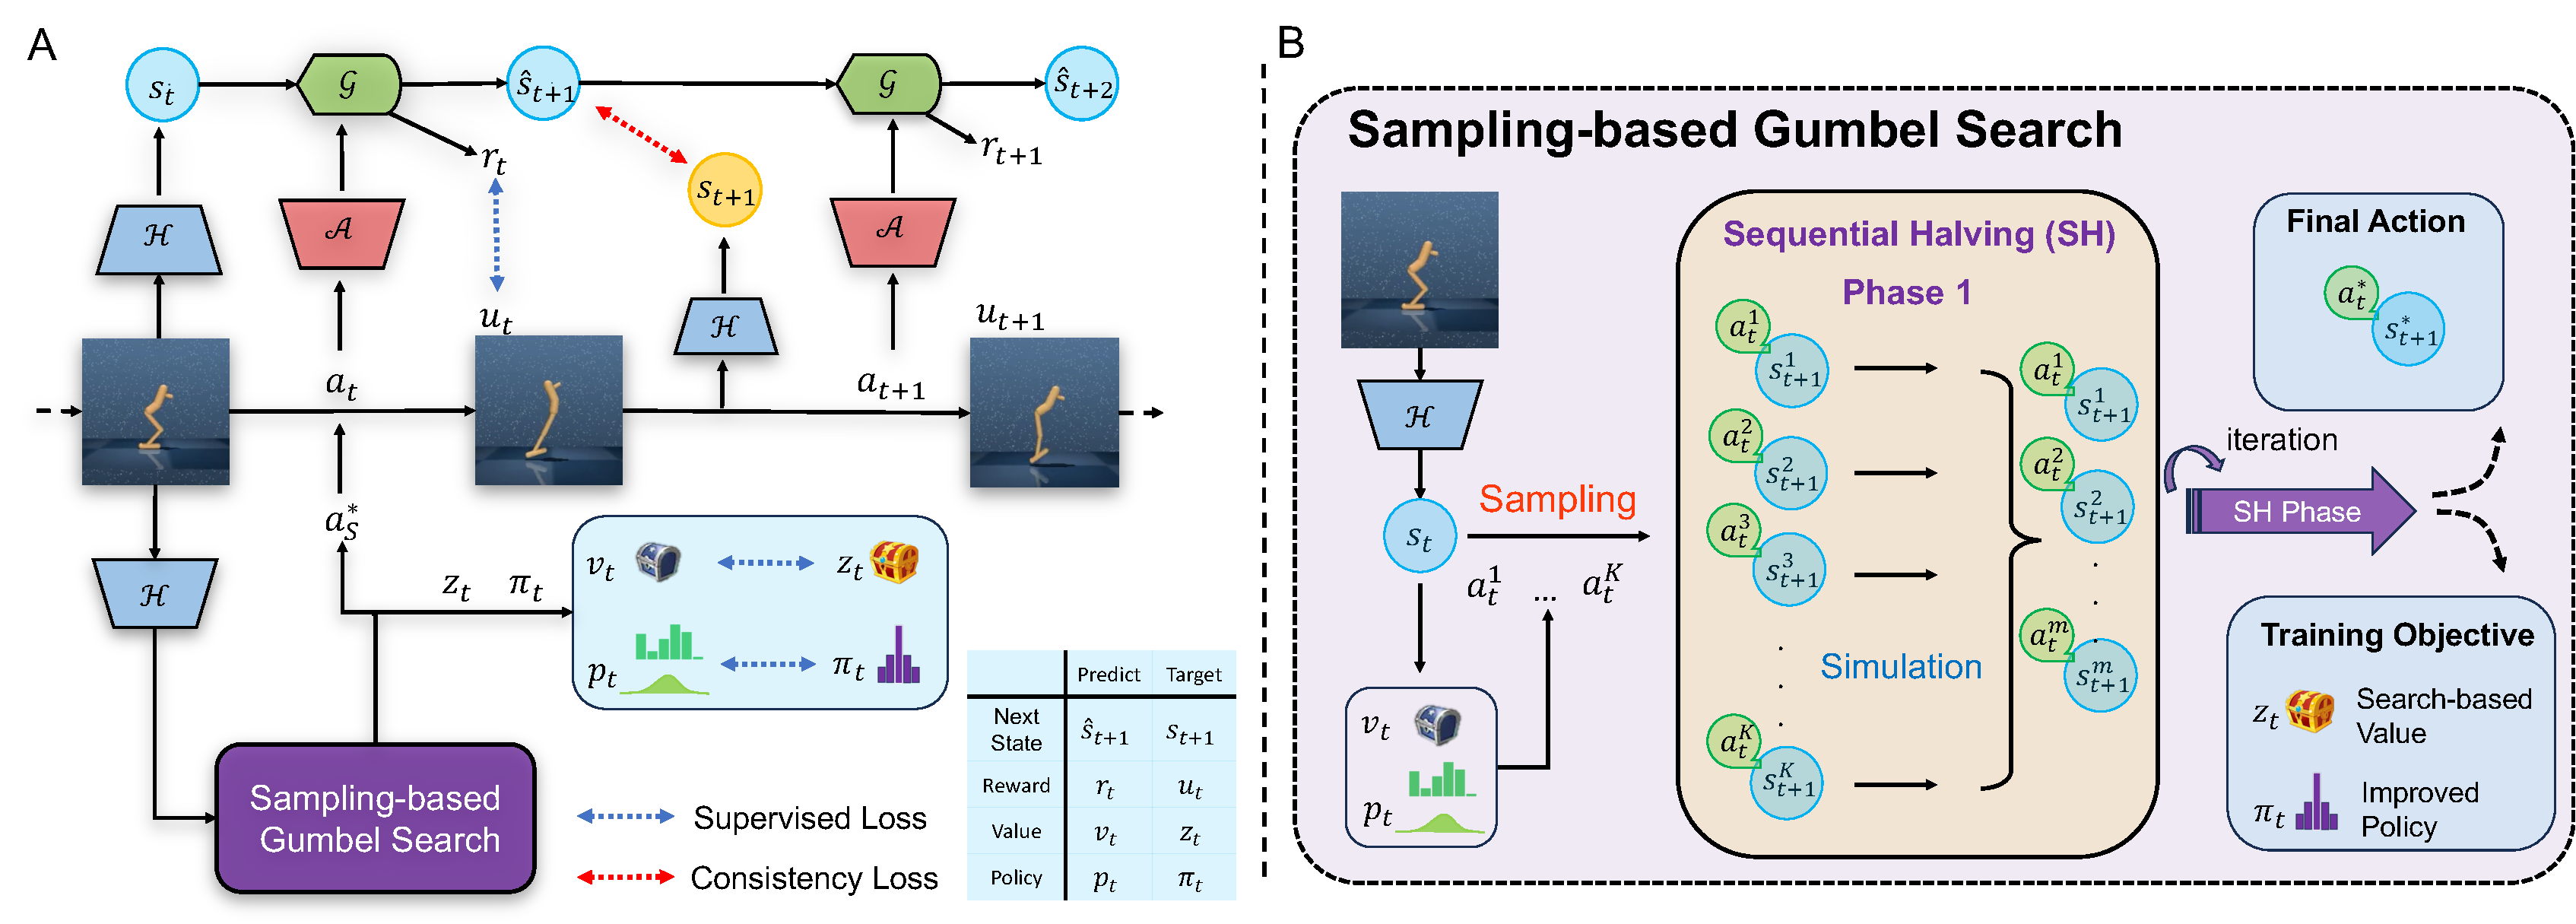
\includegraphics[width=0.98\textwidth]{sections/figs/frameworkv1.pdf}
\caption{Framework of EZ-V2. (\textbf{A}) How EZ-V2 trains its model. The representation \(\mathcal{H}\) takes observations as inputs and outputs the state. The dynamic model \(\mathcal{G}\) predicts the next state and reward based on the current state and action. Sampling-based Gumbel search outputs the target policy \(\pi_t\) and target value \(z_t\). (\textbf{B}): How the sampling-based Gumbel search uses the model to plan. The process contains action sampling and selection. The iterative action selection outputs the recommended action $a^*_S$, search-based value target (target value), and improved policy (target policy).}
\label{framework}
\end{figure*}


\section{Preliminary}

\subsection{Reinforcement Learning}
Reinforcement Learning (RL) can be formulated as a Markov Decision Process (MDP) \citep{bellman1957markovian}. An MDP in this context is formalized as a tuple \( (S, A, T, R, \gamma) \), where \( s \in S \) represents states, \( a \in A \) denotes actions, \( T: S \times A \rightarrow S \) is the transition function, \( R: S \times A \rightarrow \mathbb{R} \) is the reward function associated with a particular task, and \( \gamma \) is the discount factor. 
The goal in RL is to find an optimal policy \( \pi^* \) that maximizes the expected sum of discounted rewards over time, formally expressed as \( \max_\pi \mathbb{E} \left[ \sum_{t=0}^{\infty} \gamma^t R(s_t, a_t) \right] \), where \( a_t \) is an action taken according to the policy \( \pi \) at state \( s_t \). 
In this work, to improve sample efficiency, we learn a model of the environment during training. Meanwhile, planning with the learned model makes action selection more efficient.

\subsection{Gumbel-Top-k Trick}
\label{main_gumbel_topk}
The Gumbel-Top-k trick \citep{kool2019stochastic} can choose the top $n$ actions without replacement in a categorical distribution $\pi$. Specifically, the action sample $A$ can be sampled by the Gumbel-Max trick, which is defined as follows.
\begin{equation}
\begin{aligned}
\left(g \in \mathbb{R}^k\right) & \sim \operatorname{Gumbel}(0) \\
A & =\underset{a}{\arg \max }(g(a)+\operatorname{logits}(a)) 
\end{aligned}
\end{equation}
where $\operatorname{logits}(a)$ is the logit of the action a, and $g$ is a vector of $k$ Gumbel variables. Hereafter, we can sample $n$ actions without replacement. 
\begin{equation}
\begin{aligned}
A_1 & =\underset{a}{\arg \max }(g(a)+\operatorname{logits}(a)) \\
\vdots & \\
A_n & =\underset{a \notin\left\{A_1, \ldots, A_{n-1}\right\}}{\arg \max }(g(a)+\operatorname{logits}(a)) .
\end{aligned}
\end{equation}
Furthermore, we denote the set of $n$ top actions by $\operatorname{argtop}(g + logits, n) = {A_1, A_2,..., A_n}$.



\subsection{EfficientZero}

% Model-based learning becomes a general method to improve the sample efficiency in RL algorithms compared with model-free learning. 
% % It enhances the accuracy of action evaluation by generating potential future trajectories through a model, rather than solely relying on information from the executed trajectory. 
% EZ-V2 also benefits from the model-based learning. To achieve this, 
\subsubsection{Newtork Structure}
EfficientZero algorithm learns a predictive model in a latent space and then performs planning over actions using this model. Specifically, the components of EfficientZero consist of a representation function, a dynamic function, a policy function, and a value function, which are formulated as follows.
\begin{itemize}
    \item Representation Function:  $\mathcal{H}:s_t=\mathcal{H}(o_t)$
    \item Dynamic Function: $\mathcal{G}: \hat{s}_{t+1}, r_t =\mathcal{G}(s_t,a_t)$ 
    \item Policy Function: $\mathcal{P}:p_t=\mathcal{P}(s_t)$
    \item Value Function : $\mathcal{V}: v_t = \mathcal{V}(s_t)$
\end{itemize}
Among these components, \( o_t \) represents the current observation, \( s_t \) is the current latent state, and \( \hat{s}_{t+1} \) is the predicted next state. The representation function learns a compact state representation of the input \( o_t \). The dynamic function predicts the next state \( \hat{s}_{t+1} \) and the reward \( r_t \). 
The policy function outputs the current policy \( p_t \), and the value function provides the value estimation \( v_t \) at the current state. All components are implemented as neural networks. EZ-V2 uses a similar network structure (see Figure 2), with details of the architecture for each component provided in Appendix \ref{arch}. The main difference is that the action embedding block \( \mathcal{A} \) encodes the action \( a_t \) as a latent vector within the dynamic function.


\subsubsection{Training Process}
For the dynamic function, EfficientZero employs a supervised learning method using the true reward \( u_t \). Furthermore, EfficientZero introduces temporal consistency \citep{ye2021mastering}, which strengthens the supervision between the predicted next state \( \hat{s}_{t+1} \) and the true next state \( s_{t+1} \).
Using the learned model, an MCTS method is used for planning actions. The method can generate the target policy \( \pi_t \) and target value \( z_t \) for further supervised learning of the policy and value functions. 
Simultaneously, it outputs the recommended action \( a^*_S \) for interaction with the environment. The iterative process of interaction and training enhances the accuracy of the dynamic function's predictions and gradually improves the policy and value functions.
EZ-V2 inherits the training process of EfficientZero but replaces the MCTS method with a sampling-based Gumbel search, ensuring policy improvement in continuous action spaces. Figure \ref{framework} (A) intuitively illustrates the training process of EZ-V2.


All parameters of the components are trained jointly to match the target policy, value, and reward. 
\begin{equation}
\label{loss}
    \begin{split}
        \mathcal{L}_t &= \lambda_1\mathcal{L}_\mathcal{R}(u_t,r_t)+\lambda_2\mathcal{L}_\mathcal{P}(\pi_t,p_t)\\ &+\lambda_3\mathcal{L}_\mathcal{V}(z_t,v_t)+\lambda_4\mathcal{L}_\mathcal{G}(s_{t+1},\hat{s}_{t+1}) \\
    \end{split}
\end{equation}
where $u_t$ denotes the environmental reward, $\pi_t$ is the target policy from the search and $z_t$ represents the target value from the search. $\mathcal{L}_\mathcal{R}$, $\mathcal{L}_\mathcal{P}$ and $\mathcal{L}_\mathcal{V}$ all represent supervised learning losses.
$\mathcal{L}_\mathcal{G}$ is the temporal consistency loss \cite{schwarzer2020data}, which enhances the similarity between the predicted next state $\hat{s}_{t+1}$ with the next state $s_{t+1}$ and is formulated as: 
\begin{equation}
\label{loss}
    \begin{split}
        \mathcal{L}_{\mathcal{G}}\left(s_{t+1}, \hat{s}_{t+1}\right)&=\mathcal{L}_{cos}\left(s g\left(P_1\left(s_{t+1}\right)\right), P_2\left(P_1\left(\hat{s}_{t+1}\right)\right)\right)
    \end{split}
\end{equation}
where $\mathcal{L}_{cos}$ is the negative cosine similarity loss and $sg$ means the stop gradient operator.
The asymmetric design of employing $P_1$ and $P_2$ follows the setting in SimSiam \citep{chen2021exploring}. More details about the architecture also can be found in EfficientZero \citep{ye2021mastering}.
To enhance the prediction accuracy of the model, we unroll the loss with $l_{\text {unroll }}$ steps to train the model.
\begin{equation}
\label{loss}
    \begin{split}
    \mathcal{L} &=\frac{1}{l_{\text {unroll }}} \sum_{i=0}^{l_{\text {unroll }}-1} \mathcal{L}_{t+i} \\
    \end{split}
\end{equation}
More details of the training pipeline can be found in Appendix \ref{pipeline}.



% This involves learning to make decisions that balance immediate rewards with long-term gains, a challenge often addressed through various algorithmic strategies in RL.


% \subsection{EfficientZero}
% Our method is built on top of the EfficientZero algorithm. EfficientZero \citep{ye2021mastering} is a sample-efficient reinforcement learning approach benefited from Monte Carlo Tree Search (MCTS) and self-supervised consistency learning. As demonstrated in MuZero \citep{schrittwieser2020mastering}, MCTS serves as a general policy improvement operator with the aid of a dynamic function, a policy function, and a value function. The dynamic function consists of the reward prediction function $\mathcal{R}$ and the state transition prediction function $\mathcal{G}:r_t=\mathcal{R}(s_t,a_t), \hat{s}_{t+1}=\mathcal{G}(s_t,a_t)$, which are necessary for expanding new nodes during the search process. 
% % Like MuZero \citep{schrittwieser2020mastering}, the dynamic model of EfficientZero is learnable. The rewards and next state transitions are predicted. 
% The policy function $\mathcal{P}:p_t=\mathcal{P}(s_t)$ provides prior preferences over action candidates of a node, which helps the search concentrate on promising candidates when selecting child to expand. The value function $\mathcal{V}$, measuring the expected return of state $s_t$, provides a long-term estimation of a leaf node without further rollouts. The MCTS outputs a visit count distribution $\pi_t$ over the root node, which could be improved compared to the prior policy provided directly by the policy network. Therefore, MCTS is recognized as a policy improvement operator.
% % Additionally, EfficientZero encodes the observation as a latent state via a representation function $\mathcal{H}:s_t=\mathcal{H}(o_t)$, and operates the dynamic model, policy and value function in this hidden state space. \ywr{Introduce EZ in a messy. We should introduce the components we changed in more details.}

% Different from MuZero, EfficientZero introduces temporal consistency \cite{chen2021exploring} that strengthens the supervision in the dynamic model. This approach significantly improves the precision of state transition predictions. In summary, EfficientZero is supervised by the following losses:
% \begin{equation}
% \label{loss}
%     \begin{split}
%     \mathcal{L} &=\frac{1}{l_{\text {unroll }}} \sum_{i=0}^{l_{\text {unroll }}-1} \mathcal{L}_{t+i} \\
%         \mathcal{L}_t &= \lambda_1\mathcal{L}_\mathcal{R}(u_t,r_t)+\lambda_2\mathcal{L}_\mathcal{P}(\pi_t,p_t)\\ &+\lambda_3\mathcal{L}_\mathcal{V}(z_t,v_t)+\lambda_4\mathcal{L}_\mathcal{G}(s_{t+1},\hat{s}_{t+1})   
%     \end{split}
% \end{equation}
% where $\mathcal{L}$ is the total loss of the unrolled $l_{\text {unroll}}$ steps. Among them, $u_t$ denotes the environmental reward, $r_t$ represents the predicted reward. $\pi_t$ is the visit count distribution of MCTS. $p_t$ indicates the predicted policy priors. $z_t=\sum_{i=0}^{k-1}\gamma^i u_{t+i}+\gamma^k v_{t+k}$ represents the bootstrapped value target, and $v_t=\mathcal{V}(s_t)$ indicates the predicted value. The training architecture of EZ-V2 is similar to EfficientZero, which is indicated by Fig. \ref{framework} (A).

% \subsection{Gumbel Muzero}
% \label{gumbel_muzero}
% Our method also benefits from Gumbel MuZero \citep{danihelka2021policy} for reducing search simulations.
% Planning with Gumbel search witnesses a significant advance across a large action space under a small number of simulations.
% % Considering the limited search budgets, it leads to insufficient visits to all action candidates at the root, especially for a large action space or continuous action space. 
% % Gumbel MuZero achieves consistent policy improvement empowered by the modifications both on root action selections and non-root selections. 
% Fig. \ref{framework} (B) shows the process of Gumbel search briefly. As we can see, the process contains the action sampling, the simulation of sampled actions, the action selection based on 
% Sequential Halving (SH) \citep{karnin2013almost}. With SH repeating, we can obtain the best action $a^*_t$ finally. Furthermore, we also obtain the search-based value and improved policy at root nodes. The improved policy $\pi_t$ corresponds to the visit count distribution of MCTS.
% The simulation part expands the children of the root node to evaluate the state action pair, which is similar to that of MCTS.

% % To resolve the issue that root action candidates cannot be fully visited
% For the action sampling, Gumbel MuZero employs sampling without replacement to concentrate limited search budgets on promising candidates. To be specific, we denote the set of n top actions $\mathcal{A}_\text{topn}$ by $\operatorname{argtop}(g+\operatorname{logits}, n)$ based on Gumbel Top-k trick \citep{kool2019stochastic}, as shown in the bottom of Fig. \ref{framework} (B). $logits$ represent network-output policy priors. Gumbel noises $g$ act as exploration noises. For the action selection, Gumbel MuZero introduces Sequential Halving (SH) \citep{karnin2013almost} to replace Upper Confidence Bound (UCB) formula \citep{auer2002finite}. SH divides limited budgets into several phases, and equally visits the remaining sampled candidates within each phase to alleviate value estimation errors coming from unequal visits. At the end of each phase, SH selects the top $m$ candidates according to Gumbel scores $g_c(a)$. The formulation is $\text{argtop}(g+logits+\sigma(\hat{q}),m)$. The halving process will repeat until the search budget is used up or there is only one candidate left.

% In the simulation, Gumbel MuZero expands the non-root nodes by aligning the visit count distribution with the improved policy prior $\arg\max_{a}(\pi^{\prime}(a)-\frac{N(a)}{1+\sum_b N(b)})$.
% Inspired by reducing exploration noises in non-root nodes, the improved policy is constructed as:
% \begin{equation}
%     \pi^{\prime}=\text{softmax}(logits+\sigma(\text{completedQ}))
% \end{equation}
% where completedQ is a comprehensive value estimation of visited and unvisited candidates. For visited nodes, the completedQ is calculated via the empirical estimation as $q(a)=r(s,a)+\gamma v(s^\prime)$, $v(s^\prime)$ is the empirical mean of bootstrapped value sum and visit counts. For non-visits, $\text{completedQ}$ is estimated through weighted average Q-value of visited nodes as $\sum_{a}\pi(a)q(a)$.  
% At root nodes, the improved policy $\pi_t$
% is also obtained 
% After the search, we build a new improved policy $\pi_t$ at root nodes, which corresponds to the visit count distribution of MCTS.

% , and distill it to the policy network. 
% \ywr{We should introduce the parts concerning our modifications in detail. There is no need to describe the details implementation of the full algorithm.}